\chapter{基于异构设备处理器并行执行推断的能效优化}
\label{chapter:chapter4}

本章首先探讨了移动端SoC的发展趋势及其对深度学习模型于移动端进行离线推断的影响。通过对比分析CNN前向推断分别在手机GPU和CPU上的执行能效,\ref{chapter:chapter4-2}节详细阐述了使用移动设备上所有可获得的本地异构处理器运行CNN模型推断并非是一种高能效的方式。\ref{chapter:chapter4-3-1}节提出了一种无需人为干预、可自适应计算目标移动平台上所有本地处理器能效的算法。使用该算法可进一步获得目标移动平台上可用于执行CNN前向推断的高能效设备处理器组合。\ref{chapter:chapter4-3-2}节给出了一种为所选择设备处理器组合分配计算任务的方法。\ref{chapter:chapter4-4}节基于ODROID-XU3平台实现了本文所提出的算法,并验证了这些算法的有效性。

\section{移动端SoC的发展趋势}
\label{chapter:chapter4-1}
多核异构CPUs(如ARM的big.LITTLE\cite{chung2012heterogeneous})已然成为当前移动设备处理器的主流架构,而GPUs也已集成到绝大多数移动设备中。GPUs与生俱来的并行计算能力很适合处理深度模型中的常见计算类型。但是,处理能力较强的GPUs对移动设备的电池电量消耗也是惊人的。事实上,手机GPUs的设计过程更加重视的是低功耗而不是高性能,所以当前商业上使用的移动GPUs大部分计算能力并不是很强大,如\texttt{Mali™-T628 MP6}的最高运行频率为600MHz且核心数仅为6。因此,单独的GPUs解决方案并不能满足移动平台上深度学习模型的运行条件。

除GPUs外,移动设备中还集成了一些其他异构处理器,如DSPs、LPUs、NPUs等。高通骁龙系列SoC不仅配备了\texttt{Adreno GPU},还集成了\texttt{Hexagon DSP};英伟达Tegra K1 SoC除提供高性能的192核GPU、2.3GHz的4核CPU外,还提供了一个第五代低功耗核LPC;华为的海思麒麟970内置了神经网络处理单元(NPU),使用NPU可进行高效的AI相关计算。另外,英伟达如今已跟芯片设计公司ARM达成合作,将开源的NVIDIA深度学习加速器(NVDLA)架构集成到ARM的Project Trillium平台上,从而更好地实现移动端机器学习。在2018年的世界移动通信大会(MWC)上,联发科亦宣布推出Helio P60芯片,该芯片使用的\texttt{ARM Cortex™-A73}是专门为移动端AI应用设计的处理器架构,其可用于实现基于深度学习的面部检测、物体与场景辨识等算法。由此可见,移动端SoC将会越来越多地配备不同用途的专用处理器,并且每一种处理器都会拥有着不同的资源特征。因此,根据层的类型以及模型的资源需求差异,使用不同的处理器组合执行不同的深度学习模型必然可以带来不同的性能-功耗折中\cite{attia2015dynamic}。

\section{基于异构计算的CNN并行推断研究动机}
\label{chapter:chapter4-2}
之前的研究工作要么在CNN推断中没有很好地利用手机移动设备的异构计算能力(如仅使用CPU或GPU进行前向推断),要么总是试图利用所有可获得的本地设备处理器进行模型推断,而本章主要探索如何高能效地利用手机移动设备的异构计算能力完成CNN模型的离线推断过程。

\begin{figure}[htbp]
    \centering
    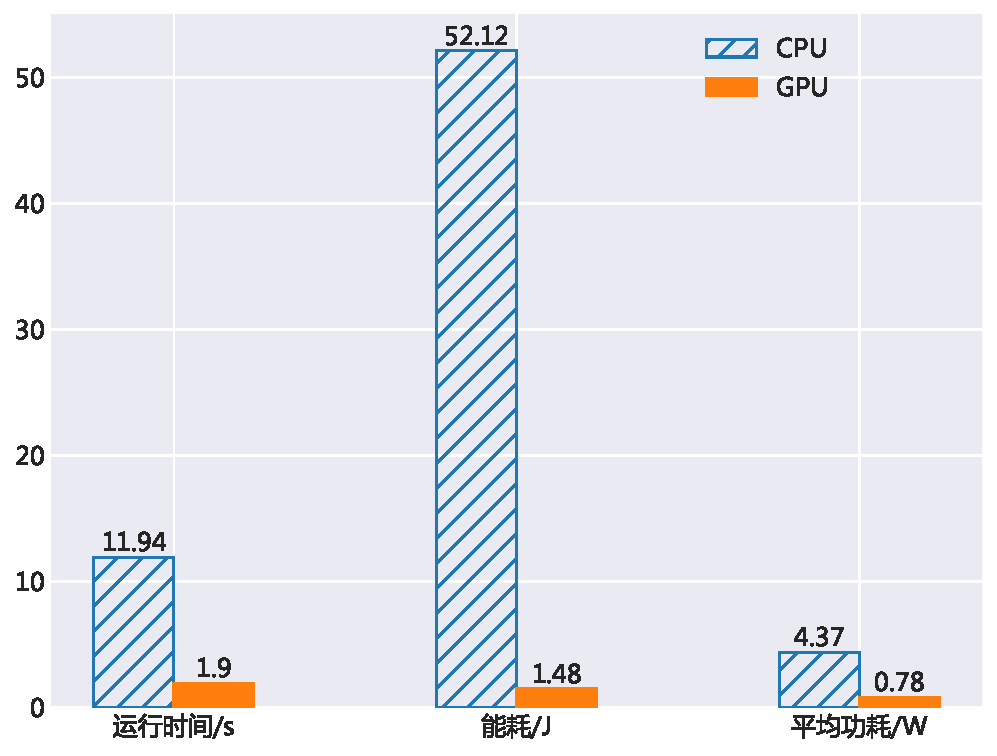
\includegraphics[height=0.4\textwidth]{figures/yolo_energy.pdf}
    \caption{手机GPU和CPU执行完整CNN推断的运行时间、能耗和平均功耗}\label{figure:figure28}
\end{figure}

图\ref{figure:figure28}显示了分别在手机GPU和CPU上运行一次完整CNN推断所需时间、能耗和平均功耗。为了充分利用手机CPU的计算性能,实验中CPU执行CNN前向推断时使用了ARM处理器提供的NEON指令(一种单指令多数据流)并且启用了与处理器核心数相同的线程。由图\ref{figure:figure28}可知,即使利用了CPU所有的并行处理能力,CPU执行一次完整的CNN前向推断过程仍需要耗时11.94秒、耗能52.12焦。然而,当使用GPU去处理相同的一次推断时,运行时间和能耗仅为1.9秒和1.48焦。由此可见,若只是一味地追求执行速度,可以同时使用手机GPU和CPU并行地执行CNN前向推断。但是,这种方式必然导致一个很低的执行能效。原因可从表\ref{table:table9}所示CPU和GPU的EDP能效值得出,即GPU的推断能效是CPU的221倍。因为手机的电池电量总是有限的,所以手机系统必须在程序执行速度与能耗开销之间维持一个良好的折中。

\begin{table}[htbp]
  \centering
  \caption{分别于手机GPU和CPU上执行一次完整CNN推断的能效}
  \label{table:table9}
  \begin{tabular}{cc}
    \toprule
      运行处理器 & EDP(Joules*seconds) \\
    \midrule
      CPU & 622.31 \\
      GPU & 2.81 \\
    \bottomrule
  \end{tabular}
\end{table}

基于上述分析,本文得出结论:不同的CNN模型在手机移动平台上执行前向推断时,需要针对性地选择一个高能效的本地异构计算组合而非简单地利用所有可获得的异构设备处理器。

\section{基于异构计算的自适应计算任务分配策略}

图\ref{figure:figure29}显示了基于异构计算的自适应计算任务分配策略的基本流程。首先,为了在目标移动平台上寻找一个可高能效并行执行CNN前向推断的异构设备处理器组合,手机应用的CNN运行时库会根据\ref{chapter:chapter4-3-1}节提出的算法自动评估本地所有不同设备处理器的能效。然后,一旦寻找到所需的设备处理器组合,CNN运行时库会根据所选择的每一个处理器的性能对计算任务进行划分,划分方法详见\ref{chapter:chapter4-3-2}节。最后,所有的计算任务会被所选择的高能效设备处理器组合并行处理。

\begin{figure}[htbp]
    \centering
    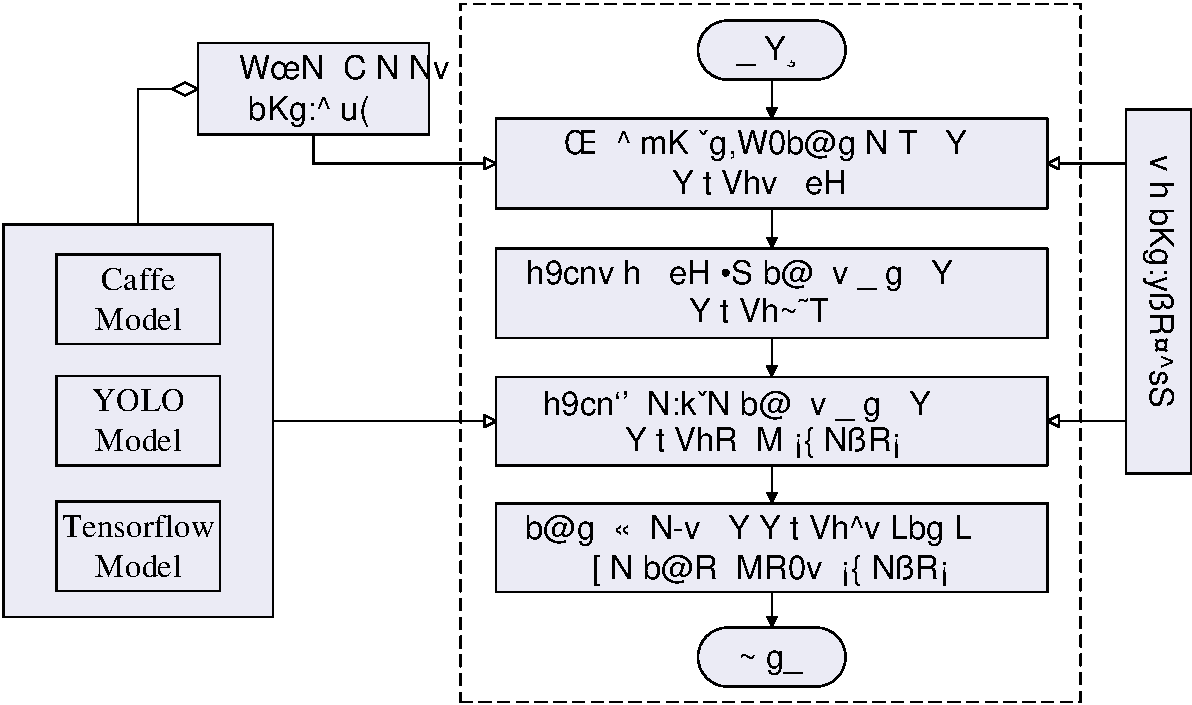
\includegraphics[height=0.4\textwidth]{figures/strategy_overview.pdf}
    \caption{基于异构计算的自适应计算任务分配策略工作流程}\label{figure:figure29}
\end{figure}

\subsection{高能效设备处理器组合的搜索}
\label{chapter:chapter4-3-1}

为了获得所期望的高能效设备处理器组合,首先需要了解目标手机移动平台上每一个可访问设备处理器的能效。本文使用一种简单有效的方法来刻画目标平台上所有设备处理器的性能和能耗。简单来说,若目标平台上所有可访问的设备处理器数量为$n$,则在CNN推断时库的前$n$次运行中,每次都仅使用一个可访问的设备处理器执行完整的CNN推断。在每次执行完CNN推断后,推断过程在该设备上所需的执行时间、能耗、平均功耗以及EDP能效值会被记录下来。这一步会造成一些运行时开销,但是它仅仅发生在程序的前若干次运行中,所以这些开销会被程序的整个运行周期所均摊。为了给接下来的搜索步骤做准备,每一个本地设备处理器的推断性能和推断功耗将会被正则化。最后,根据所期望的能效值不断剔除较低能效的设备处理器便可获得所需的高能效设备处理器组合。需要强调的是,对于同一应用,高能效设备处理器组合可被重复使用,因此整个搜索过程仅需执行一次。

\begin{algorithm}[htbp]
  \small
  \SetAlgoLined
    \begin{spacing}{0.85}
    \KwIn{(i) CNN模型结构参数和预训练的模型权重矩阵\;
          (ii) 能效阈值$EDP_{TH}$(默认值为1)。}
    \KwOut{所期望的高能效处理器组合$S_{HC}$以及组合中所有处理器的相对性能集合$Perf$。}
    遍历目标平台上所有可访问的异构设备处理器(如GPUs,CPUs,NPUs等)并将它们放入设备集合$S_{HC}$中\;
    \For{$processor_i$ \textbf{in} $S_{HC}$} {
        使用处理器$processor_i$执行一次完整的CNN推断\;
        将本次推断的执行时间$t_i$, 能耗$e_i$以及平均功耗$p_i$分别存储到$T$,$E$和$P$三个数组中\;
        使用公式\ref{equation:equation1}计算本次推断的能效$EDP_i$并将其存储在$EDP$数组中\;
    }
    找出具有最小推断执行时间的处理器$processor_{min}$\;
    将$processor_{min}$的执行时间和平均功耗分别标记为$t_{min}$和$p_{ref}$\;
    \For{$(t_i$ \textbf{in} $T)$ \textbf{and} $(p_i$ \textbf{in} $P)$} {
    计算相对性能: $perf_{ri} = \frac{t_{min}}{t_i}$,将$perf_{ri}$添加到数组$Perf$中\;
    计算相对功耗:$p_{ri} = \frac{p_{i}}{p_{ref}}$,将$p_{ri}$添加到数组$P_r$中\;
    }
    \Repeat{$edp_r < EDP_{TH}$}{
        计算相对执行时间:$t_r=\frac{1}{\sum_{perf \in Perf}perf}$\;
        计算相对总功耗:$p_{tr}={\sum_{pr \in P_r}pr}$\;
        计算相对能效EDP值:$edp_r=(p_{tr}*t_r)*t_r$\;
        \If{$edp_r \geq EDP_{TH}$}{
            找出具有最大EDP值的处理器,并记录其下标$i$\;
            从$S_{HC}$中移除$processor_i$\;
            从$Perf$中移除$perf_{ri}$\;
            从$P_r$中移除$p_{ri}$\;
        }
    }
    \textbf{return} $S_{HC}$和$Perf$\;
   \end{spacing}
  \caption{高能效设备处理器组合的搜索过程}
  \label{algo:algorithm8}
\end{algorithm}

算法\ref{algo:algorithm8}描述了在目标手机移动平台上进行高能效设备处理器组合搜索的核心过程。为了在手机本地端完成CNN前向推断过程,模型结构参数和权重矩阵的获取是必须的,这可以通过第\ref{chapter:chapter321}节提供的模型权重参数解析脚本实现。因为算法中使用了正则化处理,所以默认的能效阈值$EDP_{TH}$设置为1。当然,用户也可以根据需要配置$EDP_{TH}$的值以得到不同的能效折中。

如算法\ref{algo:algorithm8}所示,CNN推断时库首先会遍历目标平台上所有可访问的异构设备处理器,如CPUs、GPUs或NPUs等。然后,所有可获得的设备处理器被收集到一个容器中,这是整个搜索过程的初始化步骤(行1)。使用本文提出的策略,用户不需要提前测量不同设备处理器的性能和功耗。这是因为CNN推断时库在它的前几次执行中会主动对每一个可获得设备处理器的性能和功耗进行评估并进一步计算出它们的能效EDP值(行2-7)。例如,如果目标手机平台上配备有CPUs、GPUs和DSPs,那么每个设备处理器都会完整地运行一次CNN推断并且它们的执行性能和功耗等信息都将被记录下来。这个方法也可以扩展应用到新的设备处理器上,如NPUs、DianNaos\cite{chen2014diannao}等。接着,拥有最小执行时间的处理器会被挑选出来作为一个参考(行8)。通过该参考处理器的性能和功耗信息,每一个处理器的性能和功耗将被正则化(行9-12)。因为每个处理器CNN推断执行时间的倒数(即每秒处理图像数据的帧数,FPS)可反映它的推断执行性能,所以算法中处理器$processor_i$的相对性能可以通过公式$\frac{\frac{1}{t_i}}{\frac{1}{t_{min}}}=\frac{t_{min}}{t_i}$得到(行10)。

为了充分利用并行计算的优势,每一个设备处理器所分配到的计算任务量是通过考虑其性能进行动态调整的。由算法的第10行可知,参考处理器(拥有最小推断执行时间的处理器)的相对性能为1并且其他处理器的性能都小于1。因此,参考处理器的任务分配比可通过公式\ref{equation:equation2}进行计算:

\begin{equation}
     \label{equation:equation2}
     \begin{aligned}
        ratio_{ref}=\frac{1}{\sum_{perf \in Perf}perf}
     \end{aligned}
\end{equation}

\noindent 假定参考处理器的串行推断执行时间为$t_s$,则其并行处理时间为 $ratio_{ref} \times t_s$(进一步的讨论详见\ref{chapter:chapter4-3-2}节)。因为算法中使用了正则化处理,所以$t_s$可被简单地视为1。这样,整个CNN推断的相对并行处理器时间$t_r$就等于$ratio_{ref}$(行14)。显然,所选择设备处理器组合的功耗即为组合中所有处理器的功耗总和(行15)。利用上述得到的相对执行时间和功耗即可通过公式\ref{equation:equation1}计算所选择的每一个设备处理器的相对能效EDP值$edp_r$(行16)。然后,通过比较$edp_r$与目标能效阈值$EDP_{TH}$的大小,不断更新所选择的设备处理器组合。具体来说,若当前所选择设备处理器组合的能效($edp_r$)低于目标能效,则当前所选择组合中能效最低的设备处理器就会被剔除并且相应的性能和功耗数据集合也会被更新(行17-22);重复上述过程直至得到所需的高能效异构计算组合。最后,所选择的设备处理器组合以及它们的性能参数集会作为算法\ref{algo:algorithm8}的输出返回给CNN推断时库。


\subsection{计算任务的划分}
\label{chapter:chapter4-3-2}

在完成高能效设备处理器组合的搜索步骤之后,CNN推断时库就可以根据算法\ref{algo:algorithm8}的返回结果将计算任务分配到所选择的处理器上执行。为了最小化并行处理时间,必须将不同处理器之间的等待时间尽量缩小。因此,一个本地设备处理器所分配到的计算任务量应该与其性能成正比,这即是计算任务划分方法的核心思想。

对于一个给定的预训练CNN模型,本文将每一层的一个输出节点定义成一个计算任务。换言之,每一层的计算任务量等于该层的输出节点数。因此,卷积层中一个计算任务就是一个卷积操作,而全连接层中一个计算任务就是一个内积操作。图\ref{figure:figure30}显示了一个计算任务划分的示例,其中每一条红线表示一个任务划分点。

\begin{figure}[htbp]
    \centering
    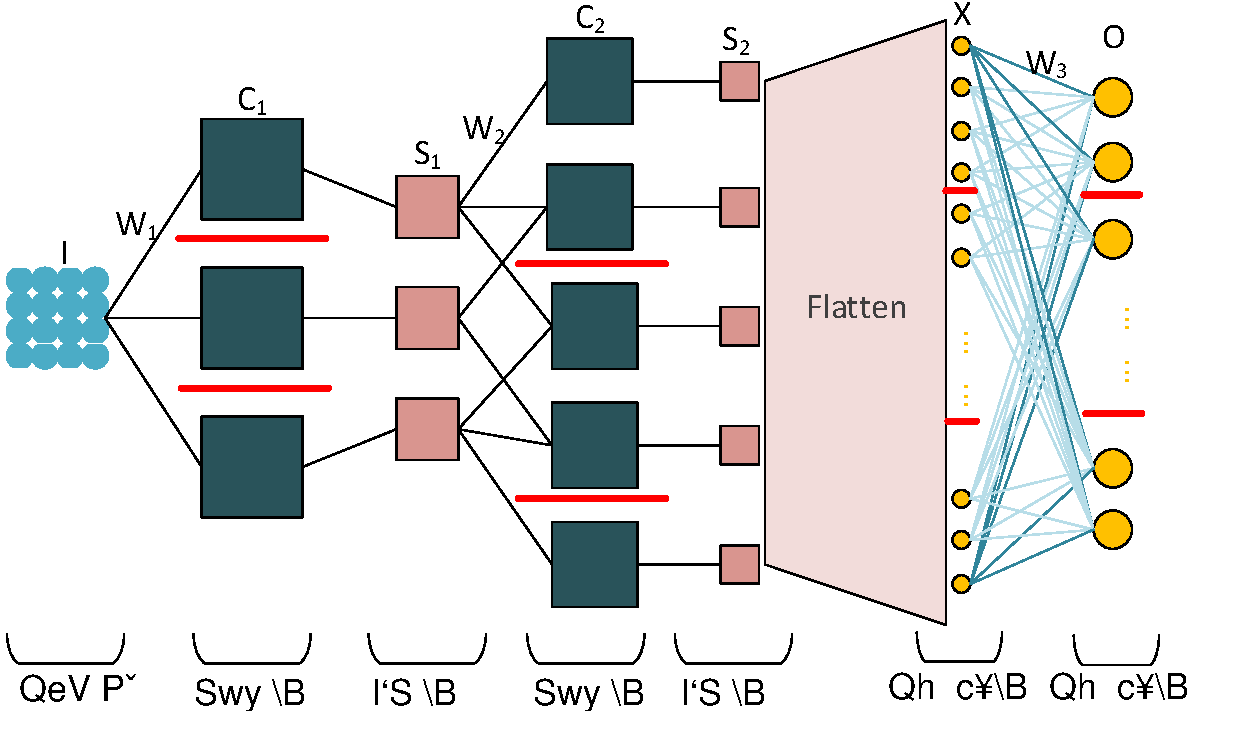
\includegraphics[height=0.4\textwidth]{figures/compute_tasks.pdf}
    \caption{计算任务划分示意图(其中每一条红线表示一个划分点)}\label{figure:figure30}
\end{figure}

算法\ref{algo:algorithm9}详细描述了为每一个所选设备处理器计算任务分配比例的方法。如前所述,分配给每一个所选设备处理器的计算任务量取决于该处理器的性能。因此,算法\ref{algo:algorithm8}输出的相对性能参数值被用来计算每一个所选设备处理器的任务分配比例(行1-4)。根据算法\ref{algo:algorithm9}输出的任务分配比例数组$R$,每一个所选设备处理器的计算任务量就可通过其任务分配比例与每一层输出节点总数的乘积获得。通过这种划分方法,性能较高的处理器就会分配到更多的计算任务而性能较低的处理器则分配到较少的计算任务。结果使得所有不同大小的计算任务几乎可以在同一时间内完成。这样,系统就可以达到一个负载平衡并在推断过程中高能效地利用平台所提供的异构计算资源。

\begin{algorithm}[htbp]
  \small
  \SetAlgoLined
    \begin{spacing}{0.85}
    \KwIn{所选设备处理器组合中所有处理器的相对性能集合$Perf$。}
    \KwOut{所选组合中处理器所分配计算任务比例集合$R$。}
    \For{$perf_{i}$ \textbf{in} $Perf$} {
        计算处理器$process_i$所分配任务比例:
        $$r_i=\frac{perf_{ri}}{\sum_{perf \in Perf}perf}$$
        将$r_i$添加到数组$R$中\;
    }
    \textbf{return} $R$\;
   \end{spacing}
  \caption{设备处理器组合中每一处理器所分配任务比例的计算过程}
  \label{algo:algorithm9}
\end{algorithm}

对于同一应用而言,算法\ref{algo:algorithm9}的执行过程只需进行一次,之后其输出的任务分配比例数组可以保存到手机本地以便重复使用。故而,算法\ref{algo:algorithm9}的运行时开销几乎可以忽略不计。


\section{实验验证}
\label{chapter:chapter4-4}
基于第\ref{chapter:chapter3}章所开发的CNN推断时库,本章进一步实现了所提出的策略并在ODROID-XU3平台上进行了实验验证。为了充分利用CPU的并行计算能力,本章也对第\ref{chapter:chapter3}章所开发的CNN推断时库进行了优化,如在CPU版本的CNN推断过程中使用了ARM处理器提供的NEON指令并且启用了与处理器核心数相同的线程。实验中,本文将CPU和GPU的运行频率保持在某一固定值(如最大运行频率),这样可以消除设备处理器运行频率的变化对实验结果的影响。

如第\ref{chapter:chapter2-5-1}节所述,ODROID-XU3平台上所有可获得的本地设备处理器包括一个CPU设备和两个GPU设备。因此,通过运行算法\ref{algo:algorithm8}和算法\ref{algo:algorithm9},CNN推断时库会得到一个高能效的设备处理器组合(这里即为ODROID-XU3平台上的两个GPU设备)。另外,实验中所考察的CNN模型主要由9个卷积层和3个全连接层构成,它们的结构参数信息如表\ref{table:table10}所示。为了说明所提策略的有效性,本文将所提策略(\emph{Our work})与贪心策略(\emph{Greedy},即总是试图使用所有可获得的异构设备处理器)进行了对比分析。

\begin{table}[htbp]
  \centering
  \caption{实验所用CNN模型的卷积层和全连接层结构参数}
  \label{table:table10}
\resizebox{1.0\textwidth}{!}{
  \begin{tabular}{ccc}
    \toprule
      名称 & 类型 & 描述\\
    \midrule
      Conv1 & 卷积层 & 输入:$3\times448\times448$,卷积核:$16\times3\times3\times3$,步长:1,padding:1,输出:$16\times448\times448$ \\
      Conv2 & 卷积层 & 输入:$16\times224\times224$,卷积核:$32\times16\times3\times3$,步长:1,padding:1,输出:$32\times224\times224$\\
      Conv3 & 卷积层 & 输入:$32\times112\times112$,卷积核:$64\times32\times3\times3$,步长:1,padding:1,输出:$64\times112\times112$ \\
      Conv4 & 卷积层 & 输入:$64\times56\times56$,卷积核:$128\times64\times3\times3$,步长:1,padding:1,输出:$128\times56\times56$\\
      Conv5 & 卷积层 & 输入:$128\times28\times28$,卷积核:$256\times128\times3\times3$,步长:1,padding:1,输出:$256\times28\times28$\\
      Conv6 & 卷积层 & 输入:$256\times14\times14$,卷积核:$512\times256\times3\times3$,步长:1,padding:1,输出:$512\times14\times14$\\
      Conv7 & 卷积层 & 输入:$512\times7\times7$,卷积核:$1024\times512\times3\times3$,步长:1,padding:1,输出:$1024\times7\times7$ \\
      Conv8 & 卷积层 & 输入:$1024\times7\times7$,卷积核:$1024\times1024\times3\times3$,步长:1,padding:1,输出:$1024\times7\times7$\\
      Conv9 & 卷积层 & 输入:$1024\times7\times7$,卷积核:$1024\times1024\times3\times3$,步长:1,padding:1,输出:$1024\times7\times7$\\
      FC10 & 全连接层 & 输入:50176, 输出:256 \\
      FC11 & 全连接层 & 输入:256, 输出:4096 \\
      FC12 & 全连接层 & 输入:4096, 输出:1470 \\
    \bottomrule
  \end{tabular}
}
\end{table}

\textbf{性能:}图\ref{figure:figure32}显示了9个卷积层和3个全连接层在ODROID-XU3平台上的执行时间。总体上来说,贪心策略的性能高于本文所提出的策略,这是因为贪心策略使用了更多的设备处理器执行计算任务。然而,贪心策略的性能提升幅度并不高,仅仅是略好于本文提出的策略,并且在全连接层上的差距非常小。这主要是因为GPUs的并行计算能力比使用了多线程和NEON指令的CPUs还要强大。由此可见,使用了一个额外CPU的贪心策略在性能上并没有表现出显著的提升。从图\ref{figure:figure32}中也可以发现贪心策略中一些层的执行时间要长于本文提出的策略。这是因为贪心策略拥有更多的任务间交互开销,其在输出节点较少的层对执行时间的影响较大。

\begin{figure}[htbp]
    \centering
    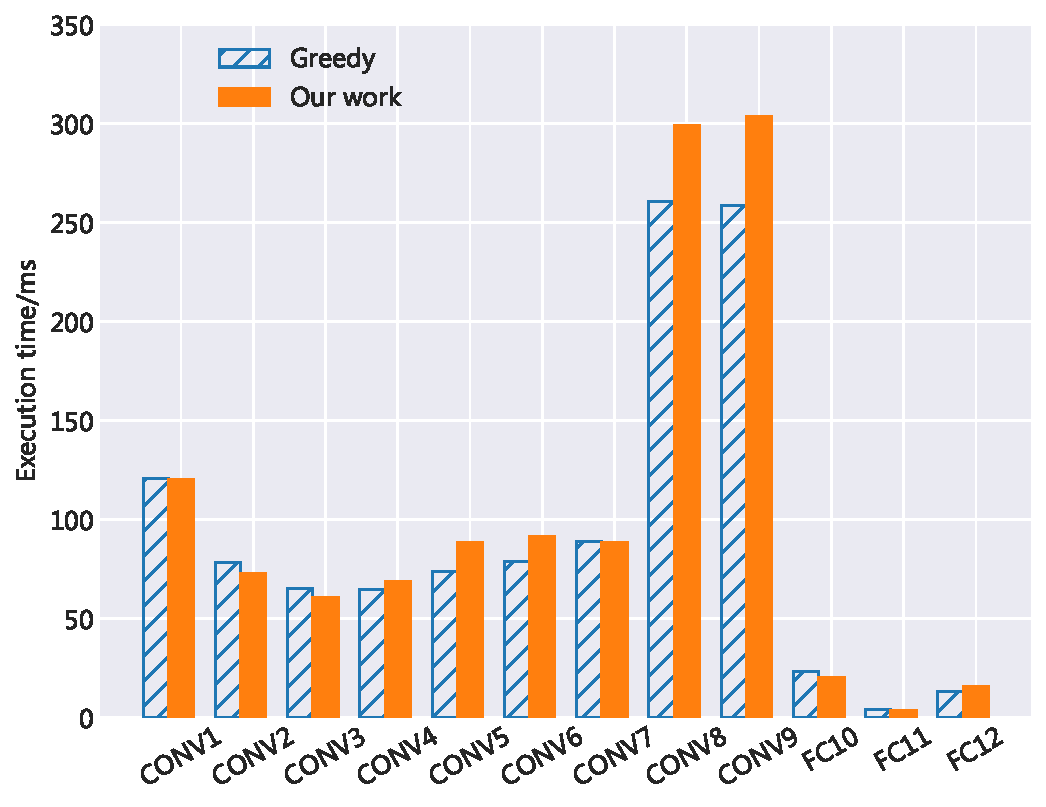
\includegraphics[height=0.4\textwidth]{figures/hc_time.pdf}
    \caption{每一层的执行时间}\label{figure:figure32}
\end{figure}

\textbf{功耗和能耗:}图\ref{figure:figure33}描述了两个策略间功耗开销对比。整体上来看,贪心策略的平均功耗约为5.44瓦而本文所提策略的平均功耗约为1.22瓦。从图\ref{figure:figure33}也可以看出,对于所有层而言,本文所提策略的功耗要远低于贪心策略的功耗。这主要是因为移动设备GPUs在设计时更多地关注低功耗而非高性能。移动GPUs通常拥有着较低的运行频率,例如:\texttt{ARM Mali-T628 MP6} GPU最大运行频率为600MHz而\texttt{Samsung Exynos5422} CPU的最大运行频率可达2GHz\cite{hardkernel.com}。

%\begin{figure}[htbp]
%\begin{minipage}[b]{.5\linewidth}
%    \centering
%    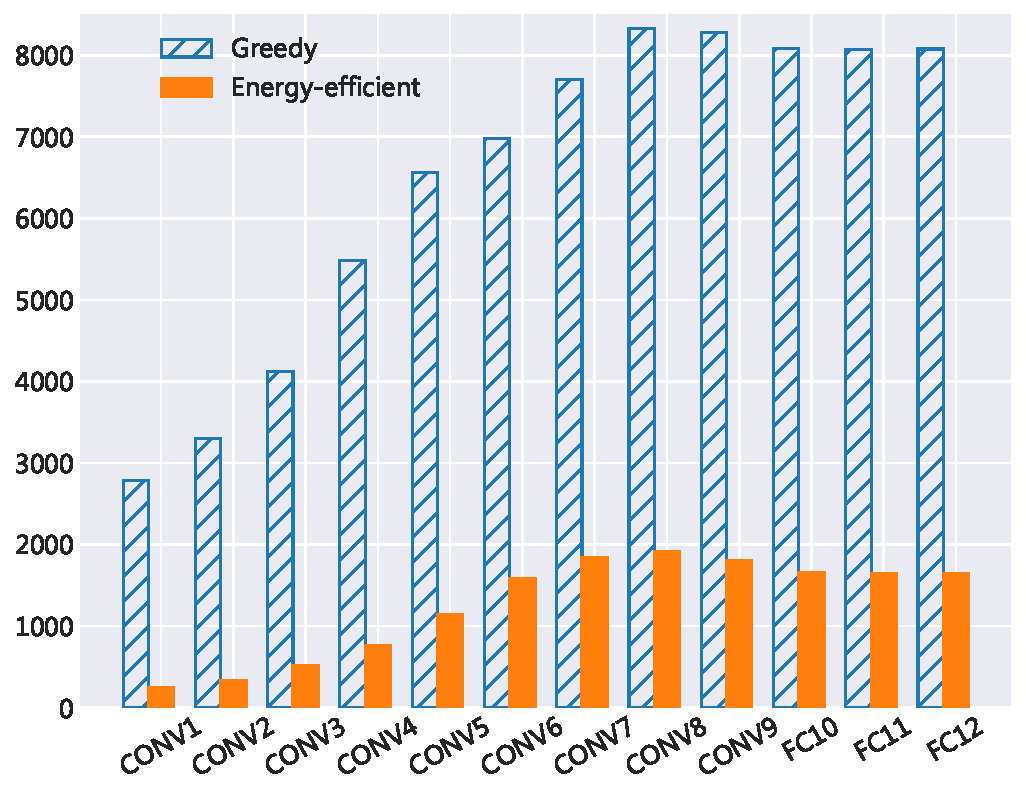
\includegraphics[height=0.75\textwidth]{figures/hc_power.pdf}
%    \caption{每一层的运行时平均功耗}\label{figure:figure33}
%\end{minipage}
%\begin{minipage}[b]{.5\linewidth}
%    \centering
%    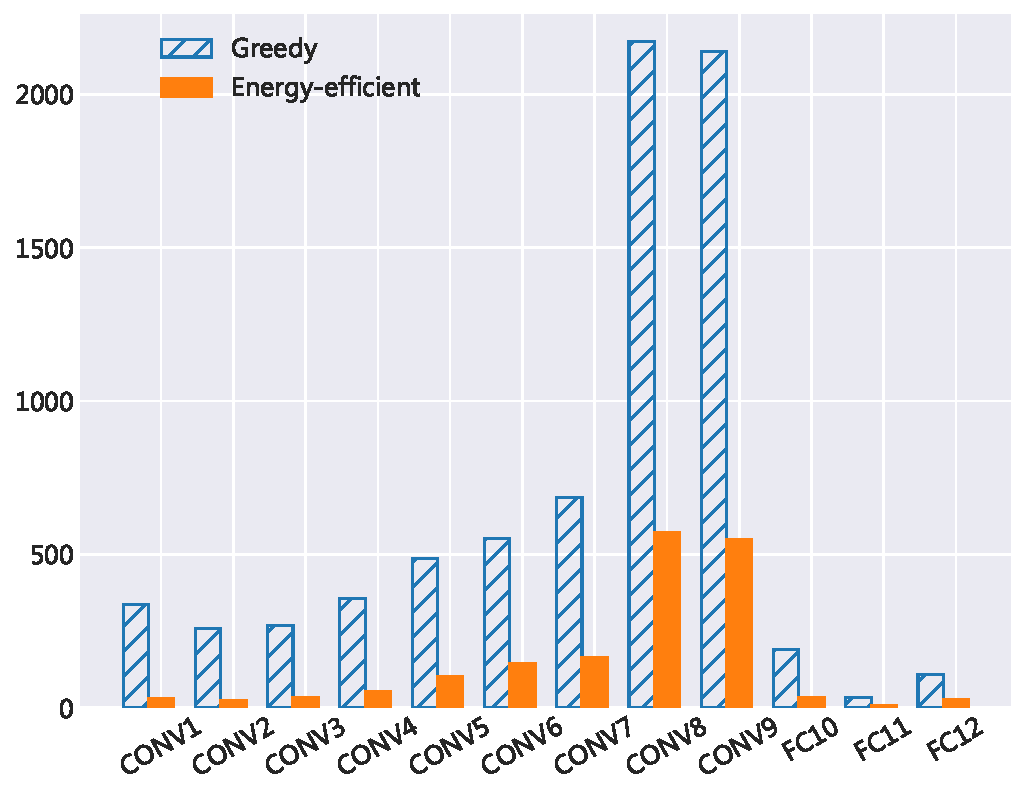
\includegraphics[height=0.75\textwidth]{figures/hc_energy.pdf}
%    \caption{每一层的运行时能耗}\label{figure:figure34}
%\end{minipage}
%\end{figure}

\begin{figure}[htbp]
    \centering
    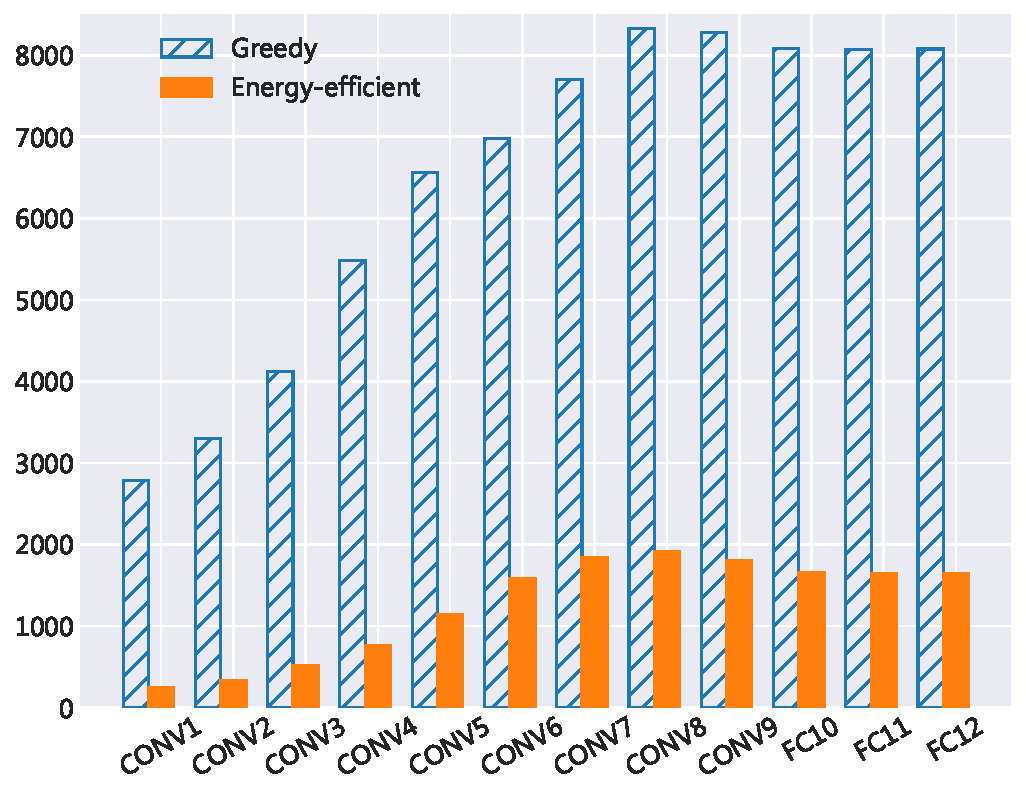
\includegraphics[height=0.4\textwidth]{figures/hc_power.pdf}
    \caption{每一层的运行时平均功耗}\label{figure:figure33}
\end{figure}

在各层的运行时能耗方面,图\ref{figure:figure34}显示了一个与功耗表现类似的趋势,即贪心策略的运行时能耗在各层上都要远高于本文所提出的策略。平均来说,贪心策略的运行时能耗约为6.59焦,而本文所提策略的能耗约为1.63焦。因此,本文所提策略通过移除一个较低能效的设备处理器有效地降低了CNN推断时的功耗和能耗。另一方面,从之前的性能分析可知,本文所提策略的推断执行性能损失很小。

\begin{figure}[htbp]
    \centering
    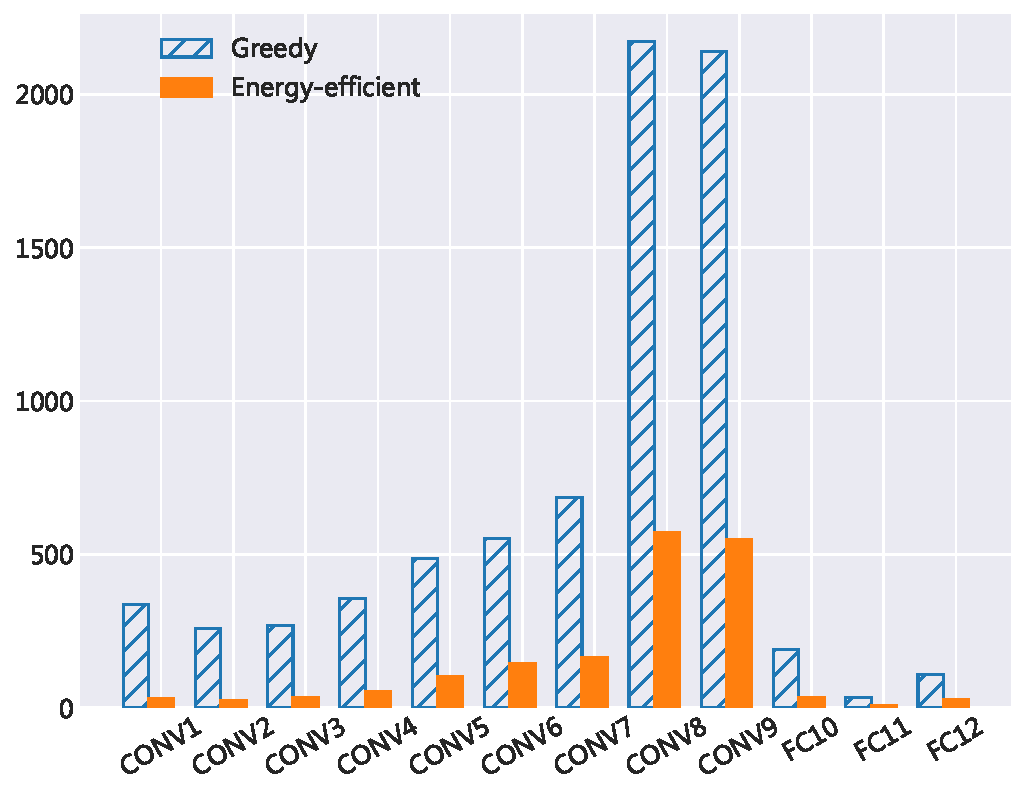
\includegraphics[height=0.4\textwidth]{figures/hc_energy.pdf}
    \caption{每一层的运行时能耗}\label{figure:figure34}
\end{figure}

\textbf{能效:}图\ref{figure:figure35}显示了不同异构计算组合执行一个完整CNN推断过程的四个方面对比,即运行时间、能耗、平均功耗和能效EDP值。\emph{Single GPU}仅使用一个GPU设备处理器执行CNN前向推断而\emph{Our work}使用由本文所提策略选择的两个GPU设备处理器并行执行CNN推断。\emph{Greedy}则使用所有可获得的设备处理器(包含一个CPU和两个GPU设备处理器)并行执行CNN推断。从柱状图\ref{figure:figure35}可以看出,随着所使用设备处理器数量的增加,CNN推断的执行时间在不断降低,而能耗和平均功耗却在逐步升高。分析EDP值可知,本文所提出的策略(\emph{Our work})拥有着更好的能效,其大约是贪心策略能效的3.67倍。与此同时,本文所提出的策略在推断执行速度上仅降低了9.7\%。

\begin{figure}[htbp]
    \centering
    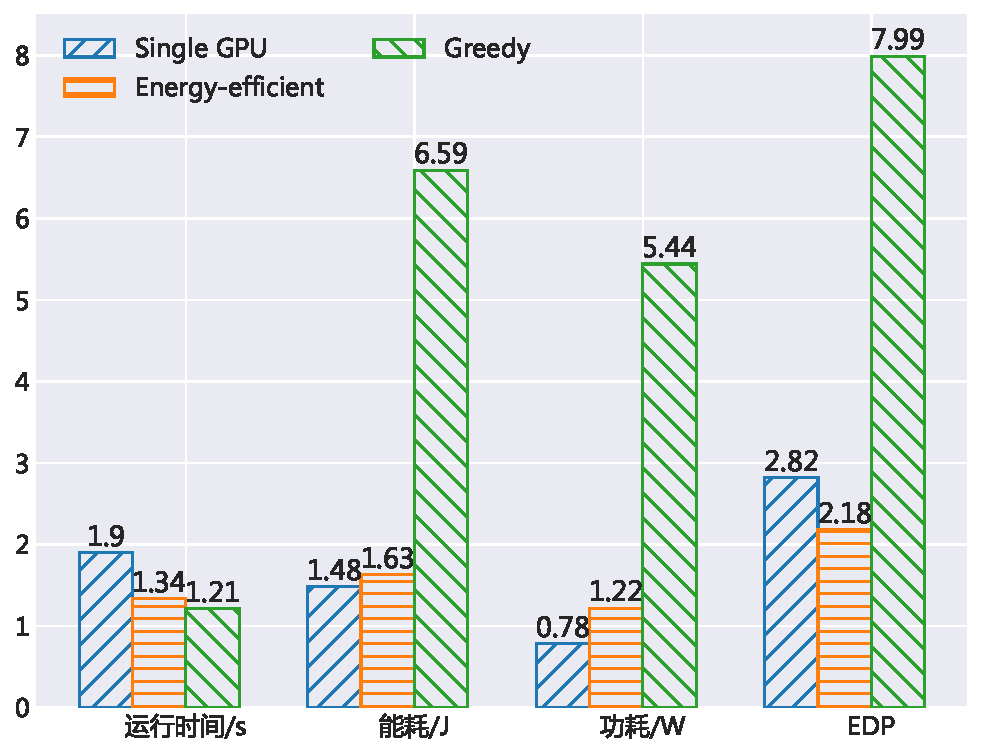
\includegraphics[height=0.4\textwidth]{figures/hc_gpu.pdf}
    \caption{不同异构计算组合的运行时间、能耗、平均功耗和能效对比}\label{figure:figure35}
\end{figure}

上述实验结果证明了利用所有可获得的设备处理器可以最大化加快CNN推断速度,但是这种方式也可能会导致一个非常低的推断能效。但是,对于电池容量受限的手机平台来说,除了需要关注程序的执行性能,程序执行过程中的能耗也是非常重要的\cite{brooks2000power}。

\section{本章小结}

尽管目前手机移动平台上并没有配备许多的异构设备处理器,但是在手机SoC上集成不同的异构处理器以执行不同的任务已经成为了一种趋势。正如\ref{chapter:chapter4-1}节所述,手机移动端的处理器架构一直在不断创新。例如,陈天石先生提出的DianNao在处理神经网络计算时执行速度是128-bit 2GHz SIMD处理器的117.87倍,并且功耗仅为485毫瓦\cite{chen2014diannao},其能效甚至超过了目前的手机GPUs。华为手机使用的麒麟970芯片即嵌入了基于DianNao架构的神经网络处理单元(NPUs)。在这种手机SoC的发展趋势下,合理高效地利用多异构设备处理器执行基于深度学习模型的手机应用将会变得越来越重要。本文对基于异构计算的移动端高能效CNN离线推断进行了探索,并对所提出的策略于ODROID-XU3平台上进行了实验验证。实验结果发现,与总是试图使用所有可获得异构设备处理器的贪心策略相比,本文所提出的策略可以将能效提升3.67倍以上而仅造成9.7\%的执行性能损失。

\cleardoublepage 